% Nguồn SGK Toán 9 Tập hai — Bài 27, trang 67--71:
% https://cdn3.olm.vn/upload/thuvienso/4491669493-page-67-1771844556727.png
% https://cdn3.olm.vn/upload/thuvienso/4491669493-page-68-1771844557069.png
% https://cdn3.olm.vn/upload/thuvienso/4491669493-page-69-1771844557385.png
% https://cdn3.olm.vn/upload/thuvienso/4491669493-page-70-1771844557693.png
% https://cdn3.olm.vn/upload/thuvienso/4491669493-page-71-1771844558020.png
% Authority: https://olm.vn/thu-vien-so/doc-sach/shs-toan-tap-2.4491669493
%
% Nguồn SBT Toán 9 Tập hai — Bài 27, PDF trang 50--51:
% SBT TOÁN 9 TẬP 2.pdf (Project Sources)
% SHA-256: 5ff01fd213d1adc75f9c54b4408d6a9642a4d8038e685040efef3311a196196c

\section{Góc nội tiếp}

\begin{lesson}
    \subsection{Kiến thức trọng tâm}

    \begin{center}
    \begin{tblr}{
        width=\linewidth,
        colspec={X[2,l] X[5,l]},
        cells={valign=t},
        row{1}={font=\bfseries, halign=c}
    }
        Khái niệm, thuật ngữ & Kiến thức, kĩ năng \\
        \begin{minipage}[t]{\linewidth}
        \begin{itemize}
            \item Góc nội tiếp
            \item Cung bị chắn
        \end{itemize}
        \end{minipage}
        &
        \begin{minipage}[t]{\linewidth}
        \begin{itemize}
            \item Nhận biết góc nội tiếp của một đường tròn.
            \item Nhận biết cung bị chắn bởi góc nội tiếp của một đường tròn.
            \item Giải thích mối liên hệ giữa số đo góc nội tiếp với số đo góc ở tâm chắn cùng một cung.
        \end{itemize}
        \end{minipage}
    \end{tblr}
    \end{center}

    Chúng ta đã biết số đo góc ở tâm $BOC$ của đường tròn $(O)$ trong Hình 9.1 bằng số đo của cung bị chắn $\widehat{BC}$. Vậy số đo của góc này có mối quan hệ gì với số đo của góc $BAC$?

    \begin{center}
    \begin{tikzpicture}
        \coordinate (O) at (0,0);
        \coordinate (A) at (90:1.65);
        \coordinate (B) at (225:1.65);
        \coordinate (C) at (315:1.65);
        \draw (O) circle (1.65);
        \draw (A)--(B) (A)--(C) (O)--(B) (O)--(C);
        \fill (O) circle (1.2pt);
        \node[above=1pt of A] {$A$};
        \node[below left=1pt of B] {$B$};
        \node[below right=1pt of C] {$C$};
        \node[above left=1pt of O] {$O$};
    \end{tikzpicture}

    \textit{Hình 9.1}
    \end{center}

    \subsubsection{Góc nội tiếp và cung bị chắn}

    \textbf{HĐ} Vẽ đường tròn tâm $O$ có bán kính bằng $2$ cm và dây cung $AB$ có độ dài bằng $2$ cm. Lấy một điểm $C$ tuỳ ý nằm trên cung lớn $AmB$ (H.9.2).
    \begin{enumerate}[label=\alph*)]
        \item Cho biết số đo của góc ở tâm $AOB$ và số đo của cung bị chắn $AB$.

        \answerline
        \item Đo góc $ACB$ và so sánh với kết quả của bạn bên cạnh.

        \answerline
        \item Lấy điểm $D$ tuỳ ý nằm trên cung $ACB$. Đo góc $ADB$ và so sánh với các góc $ACB$ và $AOB$.

        \answerline
    \end{enumerate}

    \begin{center}
    \begin{tikzpicture}
        \coordinate (O) at (0,0);
        \coordinate (A) at (225:1.55);
        \coordinate (B) at (315:1.55);
        \coordinate (C) at (105:1.55);
        \coordinate (D) at (35:1.55);
        \draw (O) circle (1.55);
        \draw (C)--(A) (C)--(B) (D)--(A) (D)--(B);
        \fill (O) circle (1.2pt);
        \node[below left=1pt of A] {$A$};
        \node[below right=1pt of B] {$B$};
        \node[above=1pt of C] {$C$};
        \node[above right=1pt of D] {$D$};
        \node[left=1pt of O] {$O$};
        \node[above right=1pt of C] {$m$};
    \end{tikzpicture}

    \textit{Hình 9.2}
    \end{center}

    $\triangle AOB$ là tam giác đều.

    Các góc $ACB$ và $ADB$ ở Hình 9.2 được gọi là các góc nội tiếp của đường tròn $(O)$ và $\widehat{AB}$ là cung bị chắn.

    Tổng quát, chúng ta có định nghĩa về góc nội tiếp như sau:

    \textbf{Định nghĩa}

    \begin{keyconcept}
        \textbf{Góc nội tiếp} của đường tròn là góc có đỉnh nằm trên đường tròn và hai cạnh chứa hai dây cung của đường tròn đó. Cung nằm bên trong góc được gọi là \textbf{cung bị chắn}.
    \end{keyconcept}

    \textbf{Ví dụ 1} Trong các góc $A$, $B$, $C$, $D$ ở Hình 9.3, góc nào là góc nội tiếp, góc nào không phải góc nội tiếp của đường tròn vẽ trong hình? Vì sao?

    \begin{center}
    \begin{tikzpicture}
        \begin{scope}[xshift=-5.1cm]
            \coordinate (Oa) at (0,0);
            \coordinate (Aa) at (-1.35,1.45);
            \coordinate (Pa) at (-1.15,-0.85);
            \coordinate (Qa) at (1.15,-0.85);
            \draw (Oa) circle (1.35);
            \draw (Aa)--(Pa) (Aa)--(Qa);
            \fill (Oa) circle (1.1pt);
            \node[above left=1pt of Aa] {$A$};
            \node at (0,-1.75) {a)};
        \end{scope}
        \begin{scope}[xshift=-1.7cm]
            \coordinate (Ob) at (0,0);
            \coordinate (Bb) at (105:1.35);
            \coordinate (Pb) at (225:1.35);
            \coordinate (Qb) at (320:1.35);
            \draw (Ob) circle (1.35);
            \draw (Bb)--(Pb) (Bb)--(Qb);
            \fill (Ob) circle (1.1pt);
            \node[above=1pt of Bb] {$B$};
            \node at (0,-1.75) {b)};
        \end{scope}
        \begin{scope}[xshift=1.7cm]
            \coordinate (Oc) at (0,0);
            \coordinate (Cc) at (-0.65,0.65);
            \coordinate (Pc) at (215:1.35);
            \coordinate (Qc) at (320:1.35);
            \draw (Oc) circle (1.35);
            \draw (Cc)--(Pc) (Cc)--(Qc);
            \fill (Oc) circle (1.1pt);
            \node[above left=1pt of Cc] {$C$};
            \node at (0,-1.75) {c)};
        \end{scope}
        \begin{scope}[xshift=5.1cm]
            \coordinate (Od) at (0,0);
            \coordinate (Dd) at (205:1.35);
            \coordinate (Qd) at (350:1.35);
            \coordinate (Rd) at ($(Dd)!-0.45!(Od)$);
            \draw (Od) circle (1.35);
            \draw (Dd)--(Qd) (Dd)--(Rd);
            \fill (Od) circle (1.1pt);
            \node[left=1pt of Dd] {$D$};
            \node at (0,-1.75) {d)};
        \end{scope}
    \end{tikzpicture}

    \textit{Hình 9.3}
    \end{center}

    \textbf{Giải}

    Các góc $A$ và $C$ không phải góc nội tiếp của đường tròn vì đỉnh không nằm trên đường tròn. Góc $D$ có một cạnh không chứa dây cung của đường tròn nên cũng không là góc nội tiếp của đường tròn. Góc $B$ có đỉnh $B$ nằm trên đường tròn và hai cạnh chứa hai dây cung của đường tròn nên là góc nội tiếp của đường tròn.

    Định lí sau cho biết mối liên hệ giữa góc nội tiếp với cung bị chắn:

    \textbf{Định lí}

    \begin{keyconcept}
        Trong một đường tròn, số đo của góc nội tiếp bằng nửa số đo của cung bị chắn.
    \end{keyconcept}

    \begin{center}
    \begin{tblr}{
        colspec={Q[c] Q[l]},
        cells={valign=m}
    }
        GT & $A,B,C\in(O)$. \\
        KL & $\widehat{ACB}=\dfrac{1}{2}\,\text{sđ}\,\widehat{AB}$ (cung $AB$ không chứa $C$). \\
    \end{tblr}
    \end{center}

    \textit{Chứng minh.} Ta xét ba trường hợp sau (H.9.4).

    \begin{center}
    \begin{tikzpicture}
        \begin{scope}[xshift=-4.2cm]
            \coordinate (Oone) at (0,0);
            \coordinate (Cone) at (110:1.35);
            \coordinate (Bone) at (290:1.35);
            \coordinate (Aone) at (215:1.35);
            \draw (Oone) circle (1.35);
            \draw (Cone)--(Aone) (Cone)--(Bone);
            \fill (Oone) circle (1.1pt);
            \node[above=1pt of Cone] {$C$};
            \node[below left=1pt of Aone] {$A$};
            \node[below right=1pt of Bone] {$B$};
            \node[right=1pt of Oone] {$O$};
            \node at (0,-1.75) {Trường hợp 1};
        \end{scope}
        \begin{scope}
            \coordinate (Otwo) at (0,0);
            \coordinate (Ctwo) at (100:1.35);
            \coordinate (Dtwo) at (280:1.35);
            \coordinate (Atwo) at (220:1.35);
            \coordinate (Btwo) at (320:1.35);
            \draw (Otwo) circle (1.35);
            \draw (Ctwo)--(Atwo) (Ctwo)--(Btwo) (Ctwo)--(Dtwo);
            \fill (Otwo) circle (1.1pt);
            \node[above=1pt of Ctwo] {$C$};
            \node[below left=1pt of Atwo] {$A$};
            \node[below right=1pt of Btwo] {$B$};
            \node[below=1pt of Dtwo] {$D$};
            \node[right=1pt of Otwo] {$O$};
            \node at (0,-1.75) {Trường hợp 2};
        \end{scope}
        \begin{scope}[xshift=4.2cm]
            \coordinate (Othree) at (0,0);
            \coordinate (Cthree) at (160:1.35);
            \coordinate (Dthree) at (340:1.35);
            \coordinate (Athree) at (220:1.35);
            \coordinate (Bthree) at (300:1.35);
            \draw (Othree) circle (1.35);
            \draw (Cthree)--(Athree) (Cthree)--(Bthree) (Cthree)--(Dthree);
            \fill (Othree) circle (1.1pt);
            \node[above left=1pt of Cthree] {$C$};
            \node[below left=1pt of Athree] {$A$};
            \node[below right=1pt of Bthree] {$B$};
            \node[right=1pt of Dthree] {$D$};
            \node[above=1pt of Othree] {$O$};
            \node at (0,-1.75) {Trường hợp 3};
        \end{scope}
    \end{tikzpicture}

    \textit{Hình 9.4}
    \end{center}

    \textit{Trường hợp 1:} Tâm $O$ nằm trên một cạnh của góc $ACB$. Giả sử $O\in CB$. Do tam giác $OAC$ cân tại $O$ và có tổng các góc bằng $180^\circ$ nên:
    \[
        2\widehat{ACB}=\widehat{ACO}+\widehat{CAO}=180^\circ-\widehat{AOC}=\widehat{AOB}.
    \]
    Do $\widehat{AOB}=\text{sđ}\,\widehat{AB}$ (vì $\widehat{AOB}$ là góc ở tâm chắn cung $AB$) nên
    \[
        \widehat{ACB}=\dfrac{1}{2}\widehat{AOB}=\dfrac{1}{2}\,\text{sđ}\,\widehat{AB}.
    \]

    \textit{Trường hợp 2:} Tâm $O$ nằm bên trong góc $ACB$. Vẽ đường kính $CD$. Áp dụng \textit{Trường hợp 1} cho các góc nội tiếp $ACD$ và $DCB$ với cạnh $CD$ đi qua $O$, ta được:
    \[
        \widehat{ACD}=\dfrac{1}{2}\,\text{sđ}\,\widehat{AD}
        \quad\text{và}\quad
        \widehat{DCB}=\dfrac{1}{2}\,\text{sđ}\,\widehat{DB}.
    \]
    Suy ra
    \[
        \widehat{ACB}=\widehat{ACD}+\widehat{DCB}
        =\dfrac{1}{2}\,\text{sđ}\,\widehat{AD}+\dfrac{1}{2}\,\text{sđ}\,\widehat{DB}
        =\dfrac{1}{2}\,\text{sđ}\,\widehat{AB}.
    \]

    \textit{Trường hợp 3:} Tâm $O$ nằm ngoài góc $ACB$. Vẽ đường kính $CD$. Áp dụng \textit{Trường hợp 1} cho các góc nội tiếp $ACD$ và $BCD$ với cạnh $CD$ đi qua $O$, tương tự như trên ta được:
    \[
        \widehat{ACB}=\widehat{ACD}-\widehat{BCD}
        =\dfrac{1}{2}\,\text{sđ}\,\widehat{AD}-\dfrac{1}{2}\,\text{sđ}\,\widehat{BD}
        =\dfrac{1}{2}\,\text{sđ}\,\widehat{AB}.
    \]

    \textbf{Nhận xét.} Từ định lí trên ta có các khẳng định sau đối với các góc nội tiếp của một đường tròn hoặc của hai đường tròn bằng nhau:
    \begin{itemize}
        \item Các góc nội tiếp bằng nhau chắn các cung bằng nhau.
        \item Các góc nội tiếp cùng chắn một cung hoặc chắn các cung bằng nhau thì bằng nhau.
        \item Các góc nội tiếp chắn cung nhỏ thì có số đo bằng nửa số đo của góc ở tâm chắn cùng một cung.
        \item Góc nội tiếp chắn nửa đường tròn là góc vuông.
    \end{itemize}

    \textbf{Câu hỏi} Hãy cho biết số đo của góc nội tiếp tìm được trong Hình 9.3 ở Ví dụ 1, biết rằng số đo của các cung màu xanh trong hình đều bằng $120^\circ$.

    \answerline

    \textbf{Ví dụ 2} Cho đường tròn $(O)$ và các điểm $A$, $B$, $C$, $D$ trên $(O)$ như Hình 9.5. Biết rằng $\widehat{BAC}=60^\circ$, hãy tính số đo của các góc $BOC$ và $BDC$.

    \textbf{Giải (H.9.5).} Xét đường tròn $(O)$, ta có:
    \begin{itemize}
        \item Do hai góc nội tiếp $\widehat{BDC}$ và $\widehat{BAC}$ cùng chắn cung nhỏ $BC$ nên
        \[
            \widehat{BDC}=\widehat{BAC}=60^\circ;
        \]
        \item Vì góc nội tiếp $\widehat{BAC}$ và góc ở tâm $\widehat{BOC}$ cùng chắn cung nhỏ $BC$ nên
        \[
            \widehat{BOC}=2\widehat{BAC}=120^\circ.
        \]
    \end{itemize}

    \begin{center}
    \begin{tikzpicture}
        \coordinate (O) at (0,0);
        \coordinate (A) at (155:1.55);
        \coordinate (B) at (55:1.55);
        \coordinate (C) at (315:1.55);
        \coordinate (D) at (225:1.55);
        \draw (O) circle (1.55);
        \draw (A)--(B) (A)--(C) (D)--(B) (D)--(C);
        \draw[dashed] (O)--(B) (O)--(C);
        \fill (O) circle (1.2pt);
        \node[left=1pt of A] {$A$};
        \node[above right=1pt of B] {$B$};
        \node[below right=1pt of C] {$C$};
        \node[below left=1pt of D] {$D$};
        \node[right=1pt of O] {$O$};
        \pic[draw, angle radius=5mm, angle eccentricity=1.35, "$60^\circ$"] {angle=B--A--C};
    \end{tikzpicture}

    \textit{Hình 9.5}
    \end{center}

    \textbf{Luyện tập} Cho đường tròn tâm $O$ và hai dây cung $AB$, $CD$ cắt nhau tại điểm $X$ nằm trong đường tròn (H.9.6). Chứng minh rằng $\triangle AXC\sim\triangle DXB$.

    \begin{center}
    \begin{tikzpicture}
        \coordinate (O) at (0,0);
        \coordinate (A) at (155:1.55);
        \coordinate (B) at (35:1.55);
        \coordinate (C) at (85:1.55);
        \coordinate (D) at (225:1.55);
        \path[name path=AB] (A)--(B);
        \path[name path=CD] (C)--(D);
        \path[name intersections={of=AB and CD, by=X}];
        \draw (O) circle (1.55);
        \draw (A)--(B) (C)--(D) (A)--(C) (D)--(B);
        \fill (O) circle (1.2pt);
        \node[above left=1pt of A] {$A$};
        \node[above right=1pt of B] {$B$};
        \node[above=1pt of C] {$C$};
        \node[below left=1pt of D] {$D$};
        \node[below right=1pt of X] {$X$};
        \node[below right=1pt of O] {$O$};
    \end{tikzpicture}

    \textit{Hình 9.6}
    \end{center}

    \answerline
    \answerline
    \answerline

    \textbf{Vận dụng} Trở lại tình huống mở đầu, hãy tính số đo của góc $BAC$ nếu biết đường tròn có bán kính $2$ cm và dây cung $BC=2\sqrt{2}$ cm.

    Tam giác $BOC$ có phải tam giác vuông không?

    \answerline
    \answerline
\end{lesson}

\begin{exercises}
    \subsection{Bài tập}

    \begin{questions}[series=SGK]
        \item Những khẳng định nào sau đây là đúng?
        \begin{questions}
            \item Hai góc nội tiếp bằng nhau thì chắn cùng một cung.
            \item Góc nội tiếp nhỏ hơn $90^\circ$ có số đo bằng nửa số đo của góc ở tâm chắn cùng một cung.
            \item Góc nội tiếp chắn cung nhỏ có số đo bằng số đo của góc ở tâm chắn cùng một cung.
            \item Hai góc nội tiếp bằng nhau thì chắn hai cung bằng nhau.
        \end{questions}

        \answerline

        \item Cho các điểm như Hình 9.7. Tính số đo các góc của tam giác $ABC$, biết rằng $\widehat{AOB}=120^\circ$, $\widehat{BOC}=80^\circ$.

        \begin{center}
        \begin{tikzpicture}
            \coordinate (O) at (0,0);
            \coordinate (A) at (155:1.55);
            \coordinate (B) at (55:1.55);
            \coordinate (C) at (320:1.55);
            \draw (O) circle (1.55);
            \draw (A)--(B)--(C)--cycle;
            \draw (O)--(A) (O)--(B) (O)--(C);
            \fill (O) circle (1.2pt);
            \node[left=1pt of A] {$A$};
            \node[above right=1pt of B] {$B$};
            \node[below right=1pt of C] {$C$};
            \node[below left=1pt of O] {$O$};
            \pic[draw, angle radius=6mm, angle eccentricity=1.35, "$120^\circ$"] {angle=A--O--B};
            \pic[draw, angle radius=4.2mm, angle eccentricity=1.45, "$80^\circ$"] {angle=B--O--C};
        \end{tikzpicture}

        \textit{Hình 9.7}
        \end{center}

        \answerline
        \answerline

        \item Cho đường tròn $(O)$ và hai dây cung $AC$, $BD$ cắt nhau tại $X$ (H.9.8). Tính số đo góc $AXB$ biết rằng $\widehat{ADB}=30^\circ$ và $\widehat{DBC}=50^\circ$.

        \begin{center}
        \begin{tikzpicture}
            \coordinate (O) at (0,0);
            \coordinate (A) at (125:1.55);
            \coordinate (B) at (65:1.55);
            \coordinate (C) at (300:1.55);
            \coordinate (D) at (210:1.55);
            \path[name path=AC] (A)--(C);
            \path[name path=BD] (B)--(D);
            \path[name intersections={of=AC and BD, by=X}];
            \draw (O) circle (1.55);
            \draw (A)--(C) (B)--(D) (A)--(D) (B)--(C);
            \fill (O) circle (1.2pt);
            \node[above left=1pt of A] {$A$};
            \node[above right=1pt of B] {$B$};
            \node[below right=1pt of C] {$C$};
            \node[below left=1pt of D] {$D$};
            \node[above=1pt of X] {$X$};
            \node[right=1pt of O] {$O$};
            \pic[draw, angle radius=4mm, angle eccentricity=1.5, "$30^\circ$"] {angle=A--D--B};
            \pic[draw, angle radius=4mm, angle eccentricity=1.5, "$50^\circ$"] {angle=D--B--C};
        \end{tikzpicture}

        \textit{Hình 9.8}
        \end{center}

        \answerline
        \answerline

        \item Cho đường tròn $(O)$ và hai dây cung $AB$, $CD$ cắt nhau tại điểm $I$ nằm trong $(O)$ (H.9.9).
        \begin{questions}
            \item Biết rằng $\widehat{AOC}=60^\circ$, $\widehat{BOD}=80^\circ$. Tính số đo của góc $AID$.
            \item Chứng minh rằng $IA\cdot IB=IC\cdot ID$.
        \end{questions}

        \begin{center}
        \begin{tikzpicture}
            \coordinate (O) at (0,0);
            \coordinate (A) at (145:1.55);
            \coordinate (C) at (205:1.55);
            \coordinate (D) at (45:1.55);
            \coordinate (B) at (325:1.55);
            \path[name path=AB] (A)--(B);
            \path[name path=CD] (C)--(D);
            \path[name intersections={of=AB and CD, by=I}];
            \draw (O) circle (1.55);
            \draw (A)--(B) (C)--(D);
            \draw (O)--(A) (O)--(C) (O)--(B) (O)--(D);
            \fill (O) circle (1.2pt);
            \node[above left=1pt of A] {$A$};
            \node[below left=1pt of C] {$C$};
            \node[above right=1pt of D] {$D$};
            \node[below right=1pt of B] {$B$};
            \node[above=1pt of I] {$I$};
            \node[below=1pt of O] {$O$};
            \pic[draw, angle radius=5mm, angle eccentricity=1.5, "$60^\circ$"] {angle=A--O--C};
            \pic[draw, angle radius=5mm, angle eccentricity=1.5, "$80^\circ$"] {angle=B--O--D};
        \end{tikzpicture}

        \textit{Hình 9.9}
        \end{center}

        \answerline
        \answerline
        \answerline

        \item Cho đường tròn $(O)$, đường kính $AB$ và điểm $S$ nằm ngoài $(O)$. Cho hai đường thẳng $SA$, $SB$ lần lượt cắt $(O)$ tại $M$ (khác $A$) và $N$ (khác $B$). Gọi $P$ là giao điểm của $BM$ và $AN$ (H.9.10). Chứng minh rằng $SP$ vuông góc với $AB$.

        \begin{center}
        \begin{tikzpicture}
            \coordinate (O) at (0,0);
            \coordinate (A) at (90:1.5);
            \coordinate (B) at (270:1.5);
            \coordinate (S) at (3.5,0.35);
            \path[name path=SA] (S)--(A);
            \path[name path=SB] (S)--(B);
            \path[name path=circlepath] (O) circle (1.5);
            \path[name intersections={of=SA and circlepath, sort by=SA, by={M,Ai}}];
            \path[name intersections={of=SB and circlepath, sort by=SB, by={N,Bi}}];
            \path[name path=BM] (B)--(M);
            \path[name path=AN] (A)--(N);
            \path[name intersections={of=BM and AN, by=P}];
            \draw (O) circle (1.5);
            \draw (S)--(A) (S)--(B) (B)--(M) (A)--(N);
            \draw (A)--(B);
            \fill (O) circle (1.2pt);
            \node[above=1pt of A] {$A$};
            \node[below=1pt of B] {$B$};
            \node[right=1pt of S] {$S$};
            \node[above right=1pt of M] {$M$};
            \node[below right=1pt of N] {$N$};
            \node[left=1pt of P] {$P$};
            \node[left=1pt of O] {$O$};
        \end{tikzpicture}

        \textit{Hình 9.10}
        \end{center}

        \answerline
        \answerline
        \answerline

        \item Trên sân bóng, khi quả bóng được đặt tại điểm phạt đền thì có góc sút bằng $36^\circ$ và quả bóng cách mỗi cọc gôn $11{,}6$ m (H.9.11). Hỏi khi quả bóng đặt ở vị trí cách điểm phạt đền $11{,}6$ m thì góc sút bằng bao nhiêu?

        % TODO(HINH-NGUON): Hình 9.11 là tranh minh hoạ sân bóng ở SGK trang 71; bổ sung asset/crop đúng từ nguồn, không redraw xấp xỉ bằng TikZ.

        \answerline
        \answerline
    \end{questions}
\end{exercises}

\begin{practice}
    \subsection{Luyện tập}

    \begin{questions}[series=SBT]
        \item Hình nào dưới đây vẽ một góc nội tiếp của đường tròn?

        \begin{center}
        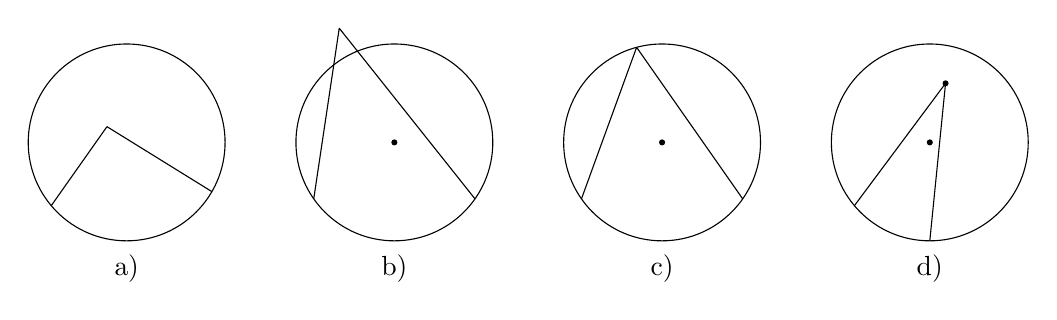
\begin{tikzpicture}
            \begin{scope}[xshift=-5.1cm]
                \coordinate (Oa) at (0,0);
                \coordinate (Va) at (-0.25,0.2);
                \coordinate (Pa) at (220:1.25);
                \coordinate (Qa) at (330:1.25);
                \draw (Oa) circle (1.25);
                \draw (Va)--(Pa) (Va)--(Qa);
                \node at (0,-1.6) {a)};
            \end{scope}
            \begin{scope}[xshift=-1.7cm]
                \coordinate (Ob) at (0,0);
                \coordinate (Vb) at (-0.7,1.45);
                \coordinate (Pb) at (215:1.25);
                \coordinate (Qb) at (325:1.25);
                \draw (Ob) circle (1.25);
                \draw (Vb)--(Pb) (Vb)--(Qb);
                \fill (Ob) circle (1.1pt);
                \node at (0,-1.6) {b)};
            \end{scope}
            \begin{scope}[xshift=1.7cm]
                \coordinate (Oc) at (0,0);
                \coordinate (Vc) at (105:1.25);
                \coordinate (Pc) at (215:1.25);
                \coordinate (Qc) at (325:1.25);
                \draw (Oc) circle (1.25);
                \draw (Vc)--(Pc) (Vc)--(Qc);
                \fill (Oc) circle (1.1pt);
                \node at (0,-1.6) {c)};
            \end{scope}
            \begin{scope}[xshift=5.1cm]
                \coordinate (Od) at (0,0);
                \coordinate (Vd) at (0.2,0.75);
                \coordinate (Pd) at (220:1.25);
                \coordinate (Qd) at (270:1.25);
                \draw (Od) circle (1.25);
                \draw (Vd)--(Pd) (Vd)--(Qd);
                \fill (Vd) circle (1.1pt);
                \fill (Od) circle (1.1pt);
                \node at (0,-1.6) {d)};
            \end{scope}
        \end{tikzpicture}

        \textit{Hình 9.3}
        \end{center}

        \answerline

        \item Cho điểm $A$ nằm trên cung lớn $BC$ của đường tròn $(O)$ và kí hiệu $\widehat{BC}$ là cung nhỏ $BC$. Vẽ bảng sau vào vở và viết số đo còn lại của góc hoặc cung tương ứng vào ô trống trong mỗi trường hợp:

        \begin{center}
        \begin{tblr}{
            colspec={Q[l] *{3}{Q[c]}},
            cells={valign=m},
            row{1}={font=\bfseries, halign=c}
        }
            & Trường hợp 1 & Trường hợp 2 & Trường hợp 3 \\
            Số đo của $\widehat{BAC}$ & $30^\circ$ & ? & ? \\
            Số đo của $\widehat{BC}$ & ? & $80^\circ$ & ? \\
            Số đo của $\widehat{BOC}$ & ? & ? & $120^\circ$ \\
        \end{tblr}
        \end{center}

        \item Cho $AB$ và $CD$ là hai đường kính của đường tròn $(O)$. Biết rằng $\widehat{AOC}=80^\circ$, tính số đo của các góc $ABC$, $ADC$ và $ABD$.

        \answerline
        \answerline

        \item Cho đường tròn $(O)$ và hai dây cung $AB$, $CD$ cắt nhau tại $X$. Tính số đo các góc của tam giác $AXC$, biết rằng $\widehat{XBD}=60^\circ$, $\widehat{XDB}=70^\circ$.

        \answerline
        \answerline

        \item Cho hai điểm $B$, $C$ nằm trên đường tròn $(O)$ và cho điểm $A$ nằm trên cung lớn $BC$. Biết rằng $\widehat{OBA}=30^\circ$, $\widehat{OCA}=40^\circ$. Tính số đo các góc của tam giác $ABC$.

        \answerline
        \answerline

        \item Cho đường tròn $(O)$ có đường kính $AB$ và điểm $C$ thuộc đường tròn sao cho $C$ khác $A$, $B$. Lấy $E$ là điểm đối xứng của $A$ qua $C$. Chứng minh rằng $BE=BA$.

        \answerline
        \answerline
        \answerline

        \item Cho tam giác nhọn $ABC$ cân tại $A$. Đường tròn đường kính $AB$ cắt các cạnh $AC$, $BC$ của tam giác $ABC$ tại $X$ và $Y$ ($X$ khác $A$, $Y$ khác $B$).
        \begin{questions}
            \item Chứng minh rằng tam giác $CXY$ cân tại $Y$.
            \item Cho $BX$ cắt $AY$ tại $K$. Chứng minh rằng $CK$ vuông góc với $AB$.
        \end{questions}

        \answerline
        \answerline
        \answerline
        \answerline
    \end{questions}
\end{practice}
